\documentclass{article}

\usepackage{wrapfig}
\usepackage{lmodern}
\usepackage[T1]{fontenc}
\usepackage[spanish]{babel}
\usepackage{mathtools}
\usepackage{graphicx}
\usepackage[utf8]{inputenc}
\usepackage{fancyhdr}



\title{Documentación \\\large \textbf{Problema Base de Datos}}
\author{Antonio Muñoz Cubero y Miguel Ángel García Mérida}
\date{22 de Ocutbre de 2020} 


\begin{document}
  \maketitle
  \pagenumbering{gobble}
  \newpage
    \section{Enunciado}
      El alcalde de una localidad nos ha contactado para que realicemos la base de datos de los clubes deportivos que hay en la localidad, puesto que necesita llevar un 
      control de estos y sus socios para mejorar en gran medida la organización de los torneos y competiciones, ya que tienen que tener regristrado todos los datos de estos. 
      Nos pide que por favor, atendamos a los siguientes supuestos:
    \\
    \\
    \textbf{Supuestos:}
    \\
      \begin{enumerate}
        
        \item Un club puede usar varias instalaciones y estas puden ser usadas por varios clubs.
        \item Las instalaciones tienen un id que las identifican, una ubicación y un deporte que para las que se usan.
        \item Un club tiene un id que lo identifica, un presidente, un nombre y un nombre oficial, una fecha de fundación, un teléfono y un correo electrónico.
        \item Los socios solo pueden pertenecer a un único club.
        \item Los socios tienen un id que los identifican, una dirección asociada, una fecha de nacimimento, el tiempo que lleva en el club, su teléfono y su correo electrónico.
        \item Existen unos afiliados, que son socios y se identifican por un identificador y tienen asociado el id de los socios, también guardaremos su teléfono y su correo.
        \item El staff técnico son socios identificados con un idStaff, id socio, tienen un rol, fecha de nacimimento y teléfono y correo.
        \item Los jugadores son socios cuyo identificativo es un id propio y también tienen el idsocio, se quiere guardar su lugar y fecha de nacimiento, la posición en la que juegan, el teléfono y su correo.
        \item Los equipos están formados por los jugadores y el staff, tienen un id cada uno, y juegan en una categoría, cada equipo tiene un nombre que puede o no ser único.
        \item Cada Equipo juega en una única categoría.
        \item Una categoría puede no tener equipos.
        \item Cada categoría puede tener ninguna o vaias competiciones.
        \item Cada categoría tiene un id que lo identifica, un nombre y un rango de edad.
        \item Cada competición tiene un id que lo identifica, una región y un número de equipos.
        \item Un miembre del staff puede pertenecer a 1 o varios equipos.
        \item Un equipo puede o no tener miembros del staff.
        \item Un jugador pertenece a un único equipo, que está compuesto por varios jugadores.
      \end{enumerate}
  \newpage    
    \section{Modelo Entidad-Relación}
      \begin{figure}[h]
        \centering
        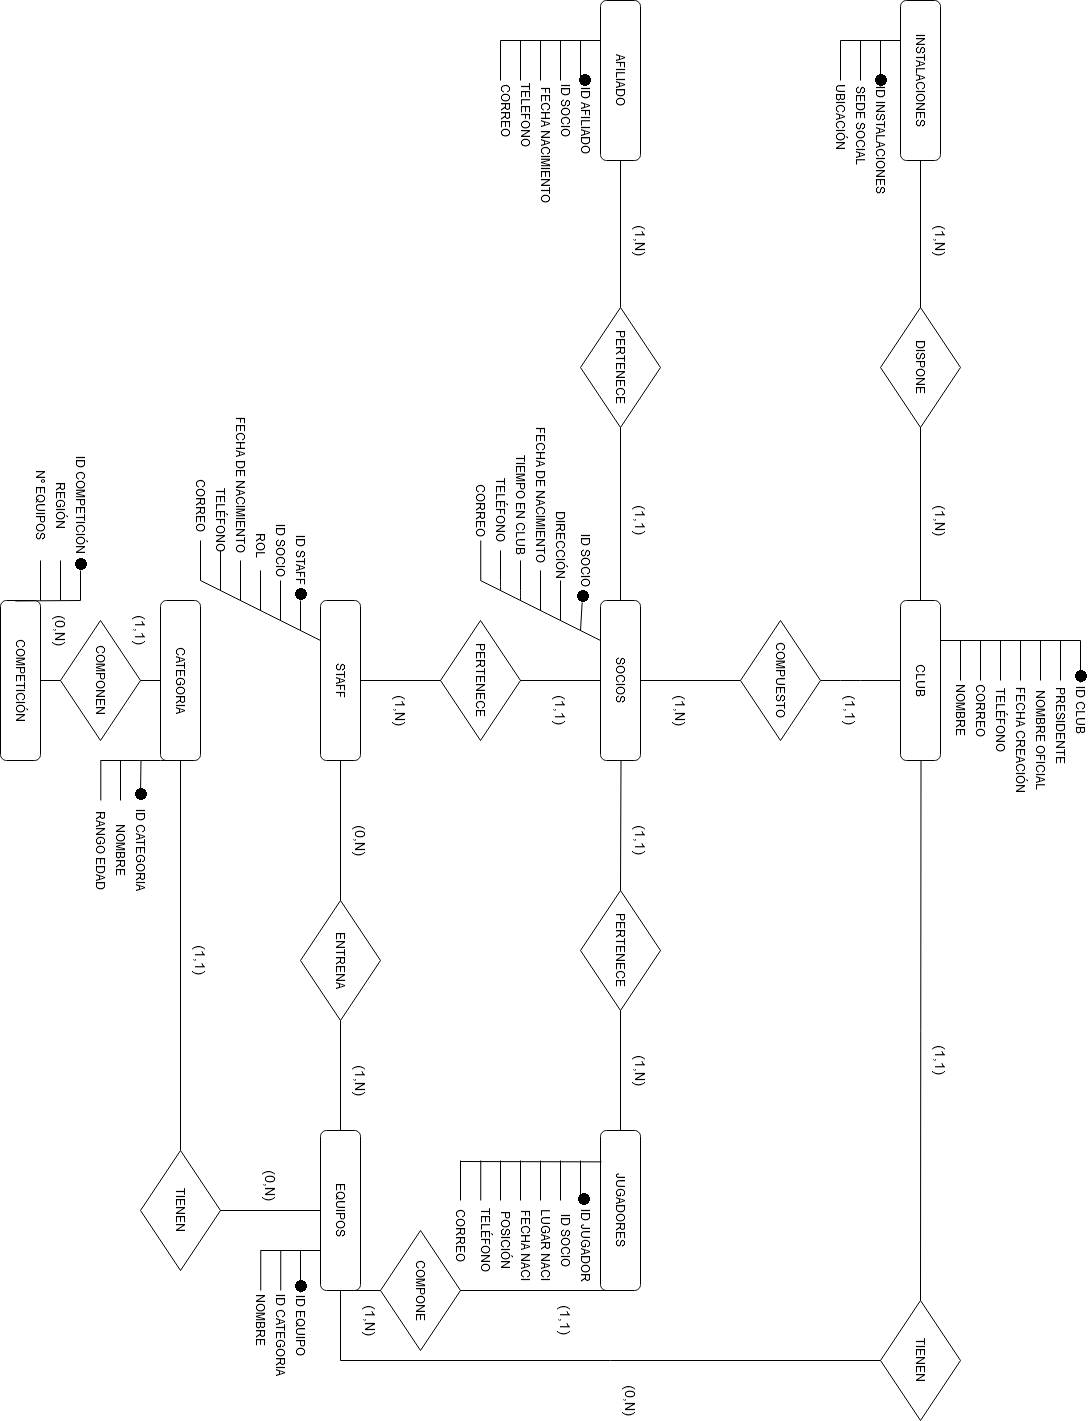
\includegraphics[scale = 0.4]{img/ClubE-R.png}
      \end{figure}

\end{document}